%\documentclass[pdftex,a4paper]{article}
\documentclass[a4paper]{article}
%%classes: article, report, book, proc, amsproc



%%%%%%%%%%%%%%%%%%%%%%%%
%% Misc

% para acertar os acentos
\usepackage[brazilian]{babel} 
% \usepackage[portuguese]{babel} 
% \usepackage[english]{babel}
% \usepackage[T1]{fontenc}
% \usepackage{aeguill}
%\usepackage[latin1]{inputenc}
\usepackage[utf8]{inputenc}
\usepackage{indentfirst}
\usepackage{fullpage}
\usepackage{appendix}
\usepackage{verbatim}
\usepackage{graphicx} %See PDF section
%%%%%%%%%%%%%%%%%%%%%%%%

% %%%%%%%%%%%%%%%%%%%%%%%%
% %% BibTeX !!
% %\usepackage{bibtex}
% \bibliographystyle{mybibtex} % .bst file
% %\bibstyle{prsty} % Choose Phys. Rev. style for bibliography

% %% Natbib
% \usepackage{natbib}
% \bibpunct{[}{]}{;}{a}{,}{,}
% %%%%%%%%%%%%%%%%%%%%%%%%

%%%%%%%%%%%%%%%%%%%%%%%%
%% PDF support

%\usepackage[pdftex]{color,graphicx}
%% Hyper-refs
%\usepackage[pdftex]{hyperref} % for printing
%\usepackage[pdftex,bookmarks,colorlinks]{hyperref} % for screen

%% \newif\ifPDF
%% \ifx\pdfoutput\undefined\PDFfalse
%% \else\ifnum\pdfoutput > 0\PDFtrue
%%      \else\PDFfalse
%%      \fi
%% \fi

%% \ifPDF
%%   \usepackage[T1]{fontenc}
%%   \usepackage{aeguill}
%%   \usepackage[pdftex]{graphicx,color}
%%   \usepackage[pdftex]{hyperref}
%% \else
%%   \usepackage[T1]{fontenc}
%%   \usepackage[dvips]{graphicx}
%%   \usepackage[dvips]{hyperref}
%% \fi

%%%%%%%%%%%%%%%%%%%%%%%%

%%%%%%%%%%%%%%%%%%%%%%%%
%% Math
\usepackage{amsmath,amsfonts,amssymb}
% para usar R de Real do jeito que o povo gosta
%\usepackage{amsfonts} % \mathbb
% para usar as letras frescas como L de Espaco das Transf Lineares
\usepackage{mathrsfs} % \mathscr

% % Theorems' labels, etc.
% \newtheorem{lema}{Lemma}[section] 
% \newtheorem{teor}[lema]{Theorem}
% \newtheorem{defi}[lema]{Definition}
% \newtheorem{prop}[lema]{Proposition}
% \newtheorem{coro}[lema]{Corolary}
% \newtheorem{exem}[lema]{Example}
% \newtheorem{apteor}{Theorem}[chapter]

% Proof commands
% \newcommand{\proofbegin}{\noindent{\bf Proof:} }
% \newcommand{\proofend}{ \hfill $\Box$ \smallskip }

% dt of integrals = \ud t
\newcommand{\ud}{\mathrm{d}}
%%%%%%%%%%%%%%%%%%%%%%%%

\usepackage{url}




%\twocolumn

\author{Felipe Figueiredo}
\title{Consultoria de Análise de Dados para Pedro Paulo Santana (Mestrado Enfermagem/UFF)}
\date{2015}

\begin{document}
\maketitle
\newpage
\tableofcontents
\listoffigures
\listoftables
\newpage
\section{Metodologia utilizada}

Em todas as análises, foi adotada a  significância de 5\%. As análises estatística foram feitas utilizando o software estatístico R, versão 3.2.2 (\url{https://www.R-project.org}).

\newpage
\section{Resultados}

\subsection{Estatísticas descritivas}

\subsubsection{Estatísticas}

\begin{table}[!h]
  \centering
  \begin{tabular}{c|ccccc}
    \hline
    Variável& Média (DP) &Mediana (AIQ)&&&\\
    \hline
    \hline
    \hline
  \end{tabular}
  \caption[Estatísticas descritivas dos dados numéricos]{Estatísticas descritivas dos dados numéricos (terminar de preencher)}
  \label{tab:descritivas}
\end{table}

As estatísticas descritivas das variáveis analisadas estão sumarizadas na tabela \ref{tab:descritivas}\ldots

\subsubsection{Gráficos}


\begin{figure}[!h]
  \centering
  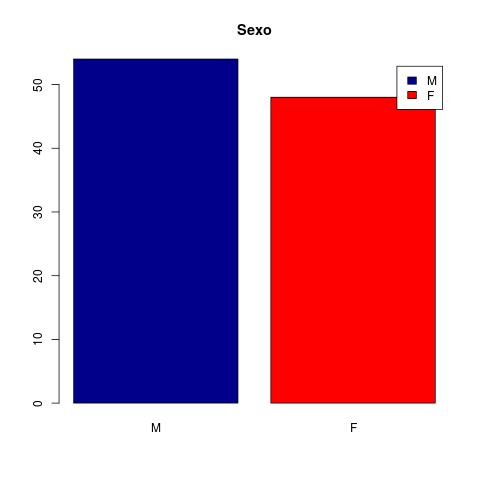
\includegraphics[width=.5\textwidth]{../figuras/sexo-bp}
  \caption{Sexo (barplot)}
  \label{fig:}
\end{figure}

\begin{figure}[!h]
  \centering
  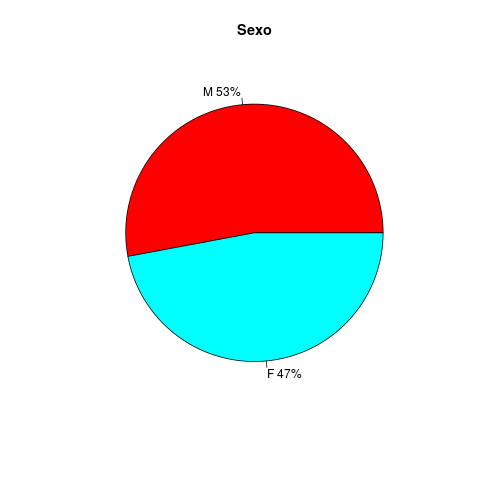
\includegraphics[width=.5\textwidth]{../figuras/sexo-pizza-pct}
  \caption{Sexo (pizza)}
  \label{fig:}
\end{figure}

\begin{figure}[!h]
  \centering
  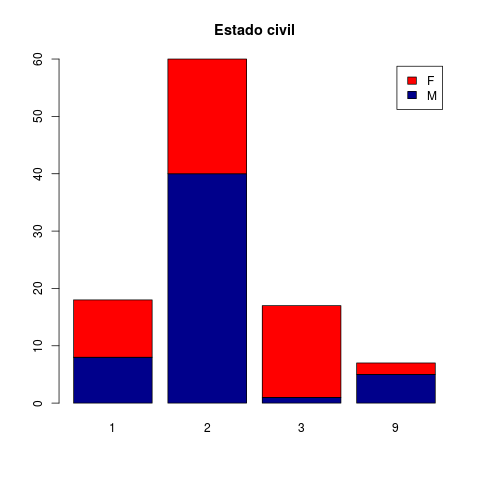
\includegraphics[width=.5\textwidth]{../figuras/est_civ-barplot}
  \caption{Estado civil, por sexo}
  \label{fig:est_civ-barplot}
\end{figure}

\begin{figure}[!h]
  \centering
  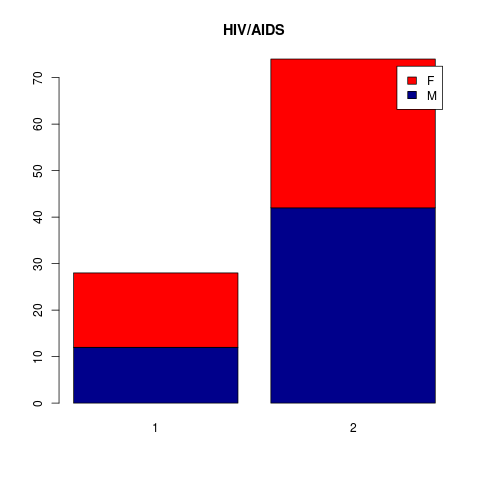
\includegraphics[width=.5\textwidth]{../figuras/hiv_aids-barplot}
  \caption{HIV ou AIDS, por sexo}
  \label{fig:}
\end{figure}

\begin{figure}[!h]
  \centering
  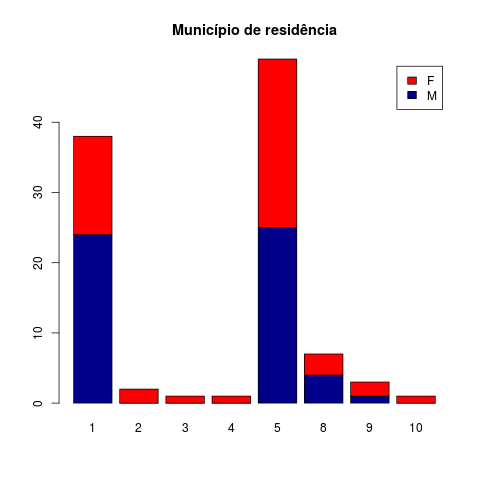
\includegraphics[width=.5\textwidth]{../figuras/muni_res-barplot}
  \caption{Município de residência, por sexo}
  \label{fig:muni_res-barplot}
\end{figure}

\begin{figure}[!h]
  \centering
  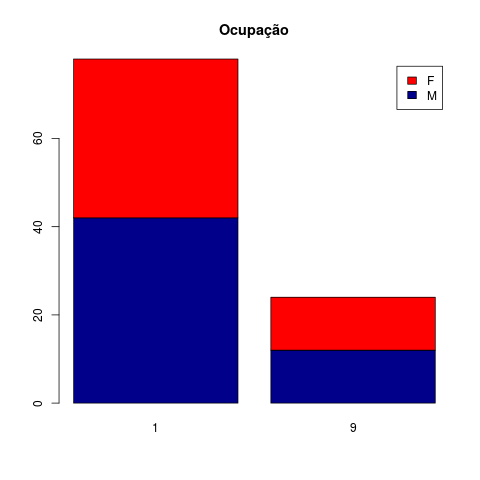
\includegraphics[width=.5\textwidth]{../figuras/ocupac-barplot}
  \caption{Ocupação, por sexo}
  \label{fig:ocupac-barplot}
\end{figure}

\begin{figure}[!h]
  \centering
  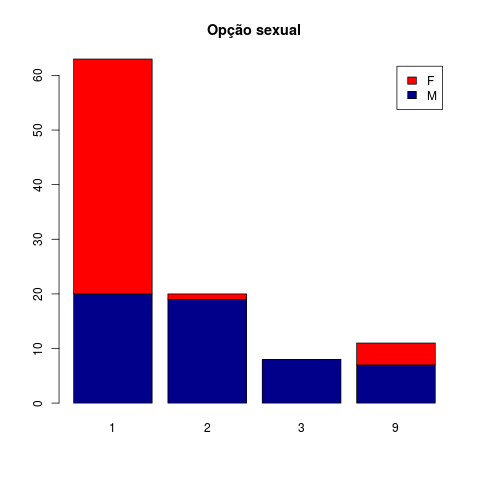
\includegraphics[width=.5\textwidth]{../figuras/opc_sex-barplot}
  \caption{Opção sexual, por sexo}
  \label{fig:opc_sex-barplot}
\end{figure}

\begin{figure}[!h]
  \centering
  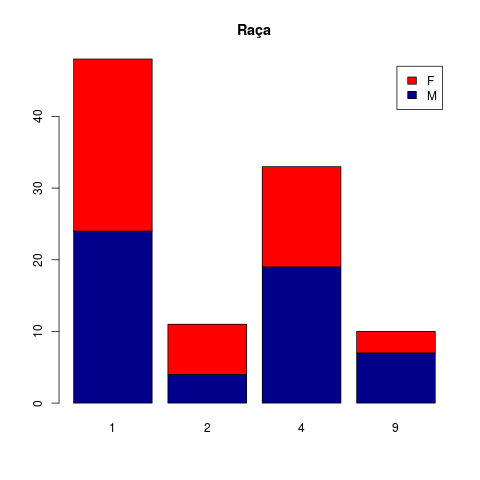
\includegraphics[width=.5\textwidth]{../figuras/raca-barplot}
  \caption{Raça, por sexo}
  \label{fig:raca-barplot}
\end{figure}

\begin{figure}[!h]
  \centering
  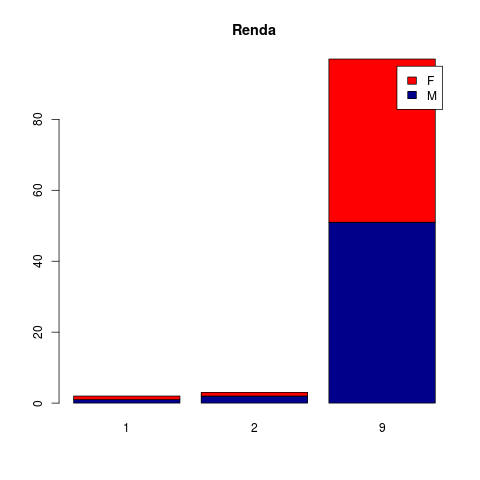
\includegraphics[width=.5\textwidth]{../figuras/renda-barplot}
  \caption{Renda, por sexo}
  \label{fig:renda-barplot}
\end{figure}

\begin{figure}[!h]
  \centering
  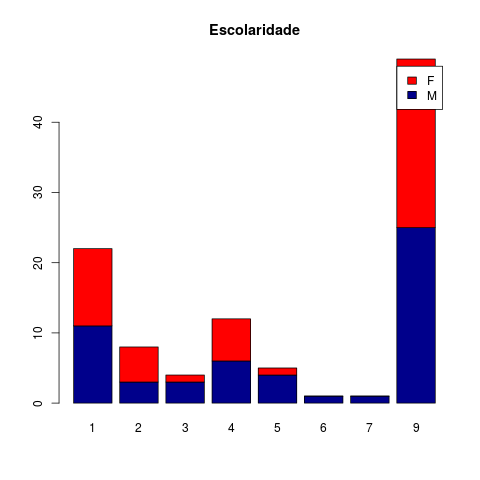
\includegraphics[width=.25\textwidth]{../figuras/escolaridade-barplot}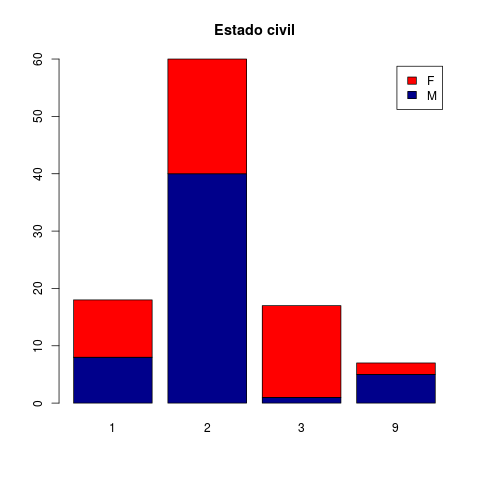
\includegraphics[width=.25\textwidth]{../figuras/est_civ-barplot}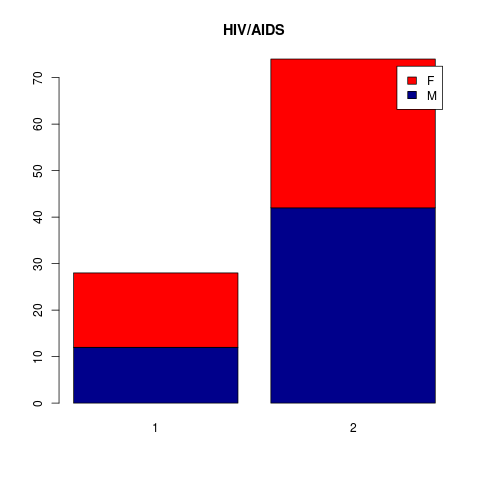
\includegraphics[width=.25\textwidth]{../figuras/hiv_aids-barplot}
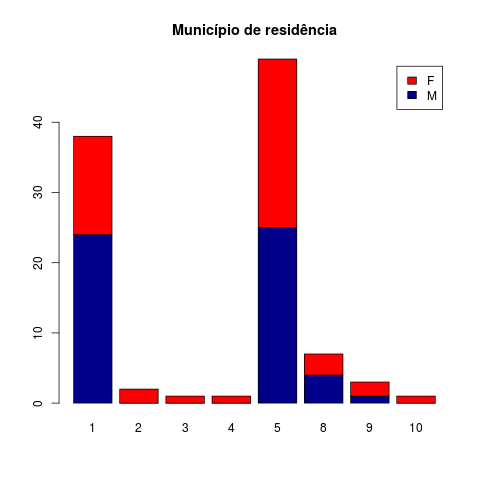
\includegraphics[width=.25\textwidth]{../figuras/muni_res-barplot}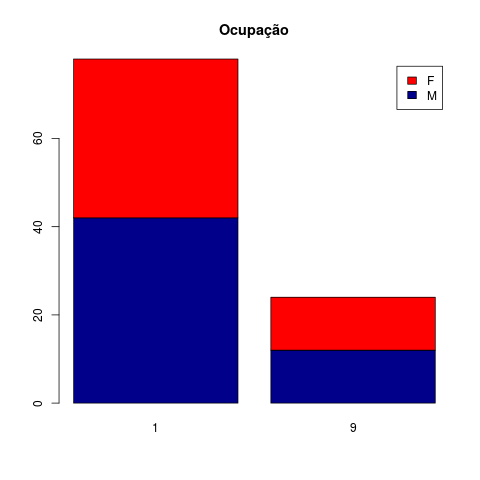
\includegraphics[width=.25\textwidth]{../figuras/ocupac-barplot}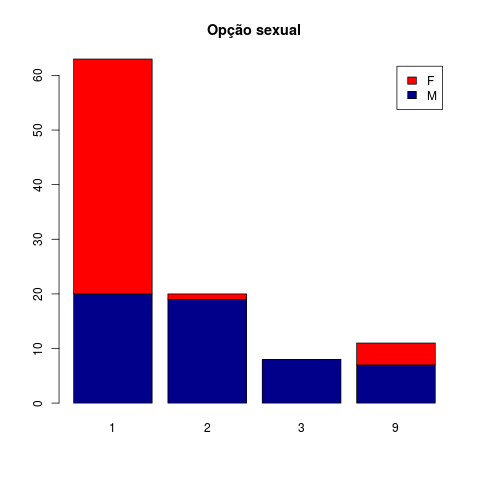
\includegraphics[width=.25\textwidth]{../figuras/opc_sex-barplot}
  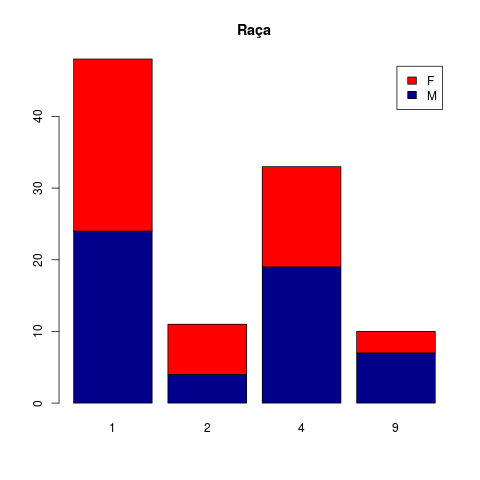
\includegraphics[width=.25\textwidth]{../figuras/raca-barplot}  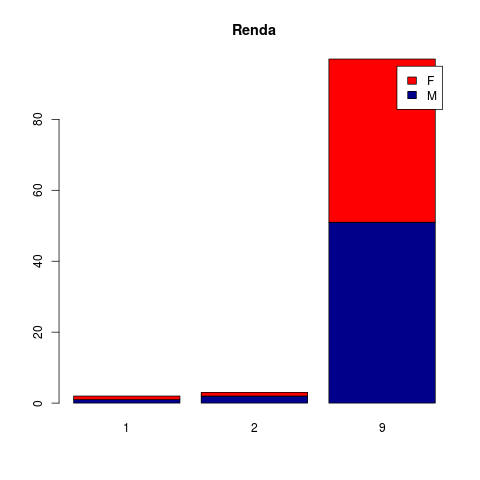
\includegraphics[width=.25\textwidth]{../figuras/renda-barplot}
  \caption{Todas as variáveis numa só figura}
  \label{fig:escolaridade-barplot}
\end{figure}



\end{document}
